\section{Load Testing Plan}
\label{se:test_plan}

In \cref{subse:modules_weather_data_integration_sys} we discussed three modules of weather data integration and assimilation systems such as integration, assimilation, and dissemination. We can map each of those modules to WDIAS modules, which provide the same functionalities as below.
\begin{enumerate}
    \item \emph{Import} modules - Integration modules
    \item \emph{Export} modules - Dissemination modules
    \item \emph{Extension} modules - Assimilation modules
\end{enumerate}

Other than the above modules, \emph{adapter modules} act as the core modules and the base of the system. Also, the \emph{query module} allows the users to query for the timeseries based on the metadata and perform Geo-based queries based on the locations.

The test plan is to perform load testing on the whole system and analyze the scalability of the system while measuring the operations performed on each module. Two variables can vary while doing performance testing.
\begin{enumerate}
    \item Number of requests made to the system at a given time (Requests Per Second (RPS))
    \item Request size
\end{enumerate}

A timeseries is a series of data points in time order. The system may receive the data points of a timeseries in multiple requests. The request size can vary based on the use case from one data point to multiple data points. For example;
\begin{itemize}
    \item A weather station may send the current water level in a regular period of 1 minute. In such a case, it always comes as a request with one data point with a higher frequency.
    \item Due to resource issues such as batteries, a weather station can collect data points for a given period and send as a batch. An example scenario would be, a weather station can collect the precipitation at each 5 minute period and send all the data after collecting for one hour.
    \item The forecast precipitation data from the \acrshort{wrf} model extract for a few days in hourly intervals and store them.
\end{itemize}

The percentage of number of requests per each data type that comes to the system at a given time can be varied depending on the situation. The Majority of weather data requests come from weather stations and other observation tools. Then we need to validate and modify those timesereis data and store them as new timeseries that can directly feed into the NWMs.. These weather stations can send the weather data at different frequencies with different parameters such as precipitation, temperature, humidity, and wind direction. Most of the timeseries mentioned above are scalar timeseries. When compared to scalar data, parameters such as wind direction are vector timeseries with a lesser percentage of requests. On the other hand, most of the grid type data was generated as results of NWMs. But those grid data produce in less frequency due to the cost of the computer resource to produce results. After considering those factors, we came up with 70\% scalar, 20\% vector, and 10\% grid percentage values at the expected requests rate ratios.
As an upper limit of such scenarios while designing the performance testing, it uses the following;
\begin{itemize}
    \item Hourly (24 data points)
    \item Every 30 minutes (48 data points)
    \item Every 15 minutes (96 data points) - One request is equivalent to a set of data points sent by a weather station in 15 minutes interval for a single day
\end{itemize}

\begin{figure}[htp]
    \centering
    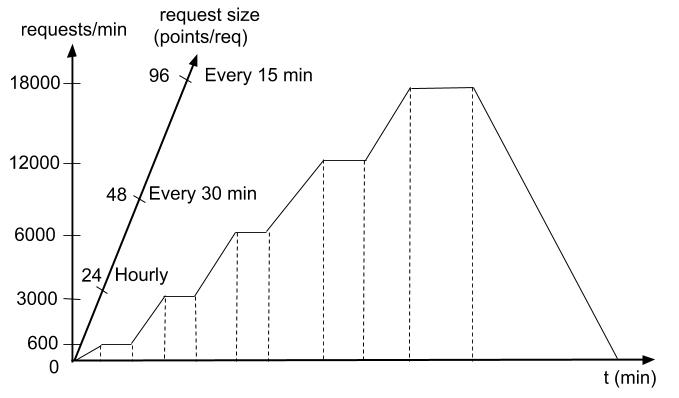
\includegraphics[width=0.8\textwidth]{results/work_load/performance_study_v4.jpg}
    \caption{\acrshort{wdias} load testing plan with changing the request size and \acrshort{rps}}
    \label{fi:performance_study_load}
\end{figure}

\cref{fi:performance_study_load} shows the summary of the load testing plan with changing the request size and performing load testing with increasing the \acrshort{rps} over time. As shown in the figure, for a given request size, the \acrshort{rps} increased in steps over the elapsed time. In each step, the \acrshort{rps} holds for a moment to give some time for the system to get stabilized. Thus at each step, we can measure the performance of the system and study the stability of the system. After the test plan comes to the peak \acrshort{rps}, the system holds for more time than the previous steps. By holding the peak load for some time, we are planning to show the system is capable of scaling more than the proposed peak load in the testing plan. During the WDIAS load testing, we are planning to have a peak of 300 requests per second at peak time. After the peak \acrshort{rps} is over, the test case goes through a cool-down period to measure the ability to shrink down the system resources when there is not any load on the system.

%%%%%%%%%%%%%%%%%%%%%%%%%%%%%%%%%%%%%%%%%%%%%%%%%%%%%%%%%%%%%%%%%%%%%%%%%%%%%%%%
\subsection{List of Test Plans}
\label{subse:test_plan_flow}
Following are the test cases which are planned to performance test cases;
\begin{enumerate}
    \item Test Setup to create timeseries in 1hr, 30min and 15min intervals and create metadata of the timeseries
    % \item Extensions
    % \begin{itemize}
    %     \item Create Extensions for /Aggregation\_Accumulative, /Interpolation Linear, /Validation Missing Values (OnChange and OnTime)
    %     \item Plan for the 15 minutes of test run with the request size of 15min data. (total 0.25 hours)
    %     \item Do with Import Timeseries with error data which will go through extensions.
    % \end{itemize}
    \item Import + Extension + Export + Timeseries Queries
    \begin{itemize}
        \item Plan for 30 minutes of the test run with the request size of 1hr (60min) data.
        \item Plan for 30 minutes of the test run with the request size of 30min data.
        \item Plan for 30 minutes of the test run with the request size of 15min data.
        \item Plan for 30 minutes of the test run with the request size of 15min data with auto-scaling.
        % \item Test plan run against 60min, 30min and 15min request size of data. Another test plan runs with enabling the auto-scaling. (total of 2 hours)
    \end{itemize}
    \item Query
    \begin{itemize}
        \item Query Timeseries
        \item Plan for the 5 minutes of test run.
    \end{itemize}
\end{enumerate}


%%%%%%%%%%%%%%%%%%%%%%%%%%%%%%%%%%%%%%%%%%%%%%%%%%%%%%%%%%%%%%%%%%%%%%%%%%%%%%%%
\subsection{Performance Metrics}
\label{subse:test_plan_metrics}

During the performance analysis, we used the following metrics to measure the performance of the system.
\begin{itemize}
    \item \emph{Throughput} -- Number of requests that can be processed per unit time. 
    Normally for \acrshort{wdias} performance observations, it uses \acrfull{rps} to measure the throughput.
    \item \emph{Latency} -- Taken time to respond to the request sent to the system. 
    Normally we measure with milliseconds (ms) in the \acrshort{wdias}. During the performance analysis, we measure the minimum response time, maximum response time, the average response time, and standard deviation. The standard deviation measures the mean distance of the values to their average value. It gives an idea of the dispersion or variability of the measures to their mean value. So, if the deviation value is low compared to the mean value, it will indicate that the measures are not dispersed (or mostly close to the mean value), and the mean value is significant. Other than that, we measure the response time into 90\% percentile while giving the best response time up to 90\% percent of the responses.
    \item \emph{Resource utilization} -- Resource Utilization is calculated based on the CPU and Memory usage via the K8s metrics server. It calculates the resource utilization over a 60 seconds time window. Network usage is getting based on the actual physical machines.
    \item \emph{Auto-scaling} -- We performed the load testing with two system configurations. First, we ran the microservices with a fixed number of pods inside the K8s cluster. Then k8s are only allowed to vertically scale each microservice until a container hits the CPU and memory limits defined per container or overwhelm the physical node resources. Secondly, we ran the load testing with auto-scaling enabled only for microservices, which are using higher resources with the above system configurations. Auto-scaling spawns new copies of the same microservice when the microservice gets more load than the configured percentage, and shrink the running instances when there is a lesser load.
\end{itemize}
